% =============================================================
%  Chapitre 4 — Réalisation et développement
% =============================================================
\chapter{Réalisation et développement}

\section*{Introduction}
Ce chapitre couvre le développement de Telnet Test Manager. On commence
par l'environnement de travail et la structure des projets, puis on
détaille l'implémentation des modules principaux~: moteur Telnet,
\gls{api} REST et connexion MongoDB.

% -----------------------------------------------------------------
\section{Environnement de développement}
% -----------------------------------------------------------------

\begin{table}[H]
  \centering
  \caption{Environnement de développement}
  \label{tab:env_dev}
  \begin{tabularx}{\textwidth}{|L{3.5cm}|L{4cm}|X|}
    \hline
    \textbf{Outil} & \textbf{Version} & \textbf{Rôle} \\
    \hline
    Visual Studio Code & 1.90+ & Éditeur de code principal \\
    \hline
    Node.js & 20 LTS (Alpine) & Environnement d'exécution JavaScript \\
    \hline
    npm & 10+ & Gestionnaire de paquets \\
    \hline
    MongoDB & 7.0 & Base de données documentaire \\
    \hline
    MongoDB Compass & 1.42+ & Client graphique MongoDB \\
    \hline
    Docker Desktop & 4.30+ & Gestion des conteneurs locaux \\
    \hline
    Postman & 11+ & Test et documentation de l'API REST \\
    \hline
    Git & 2.45+ & Contrôle de version \\
    \hline
    GitHub & --- & Hébergement du dépôt et CI/CD \\
    \hline
  \end{tabularx}
\end{table}

% -----------------------------------------------------------------
\section{Structure du projet}
% -----------------------------------------------------------------

\subsection{Structure du backend}

\begin{figure}[H]
  \centering
  \begin{lstlisting}[basicstyle=\ttfamily\small, frame=single, backgroundcolor=\color{gray!6}]
backend/
|-- src/
|   |-- domain/
|   |   |-- entities/       (User, Poste, Produit, Slot, Reference,
|   |   |                    TestResult, TelnetCommand, AuditLog, Report)
|   |   `-- repositories/   (IUserRepo, IPosteRepo, ISlotRepo, ...)
|   |-- application/
|   |   `-- usecases/       (auth/, poste/, produit/, slot/,
|   |                         reference/, test/, admin/, report/)
|   |-- infrastructure/
|   |   |-- database/       (models/, repositories/)
|   |   |-- telnet/         (TestWorkerManager.js, testWorker.js)
|   |   `-- metrics/        (prometheusMetrics.js)
|   `-- interfaces/
|       |-- http/           (controllers/, routes/, middlewares/)
|       `-- websocket/      (WebSocketServer.js)
|-- server.js
|-- package.json
`-- Dockerfile
  \end{lstlisting}
  \caption{Structure du projet backend (Clean Architecture)}
  \label{fig:backend_structure}
\end{figure}

\subsection{Structure du frontend}

Le frontend suit les conventions de \textbf{Create React App} avec
TypeScript. Un module \texttt{i18next} gère l'internationalisation et
un service API centralisé gère tous les appels HTTP~:

\begin{figure}[H]
  \centering
  \begin{lstlisting}[basicstyle=\ttfamily\small, frame=single, backgroundcolor=\color{gray!6}]
frontend/src/
|-- components/
|   |-- Login.tsx / Login.css
|   |-- Dashboard.tsx / Dashboard.css
|   |-- MultiTest.tsx / MultiTest.css
|   |-- Commands.tsx / Commands.css
|   |-- Configuration.tsx / Configuration.css
|   |-- Reports.tsx / Reports.css
|   |-- AdminPanel.tsx / AdminPanel.css
|   `-- LanguageSwitcher.tsx
|-- services/
|   `-- api.ts              (Axios + intercepteurs JWT)
|-- hooks/
|   `-- usePermissions.ts   (extraction des permissions RBAC)
|-- i18n/
|   |-- config.ts
|   `-- locales/            (fr/, en/, pt-BR/)
|-- App.tsx
`-- index.tsx
  \end{lstlisting}
  \caption{Structure du projet frontend (React + TypeScript)}
  \label{fig:frontend_structure}
\end{figure}

% -----------------------------------------------------------------
\section{Implémentation du module de test Telnet}
% -----------------------------------------------------------------

\subsection{Architecture Worker Threads}

Le moteur Telnet utilise les \textbf{Worker Threads} de Node.js pour
isoler chaque session Telnet dans un fil d'exécution séparé. Ce choix
présente trois avantages concrets~:

\begin{enumerate}
  \item \textbf{Non-blocage}~: le fil principal Express reste réactif
        aux nouvelles requêtes HTTP pendant qu'un test s'exécute~;
  \item \textbf{Isolation}~: un crash dans un Worker ne fait pas tomber
        le serveur~;
  \item \textbf{Parallélisme}~: plusieurs Workers peuvent tourner
        simultanément, permettant le module MultiTest.
\end{enumerate}

\subsection{Gestionnaire de Workers (TestWorkerManager)}

\texttt{TestWorkerManager} est un singleton qui maintient une
\texttt{Map<testId,~Worker>} permettant de retrouver et d'arrêter n'importe quel
Worker actif. La méthode \texttt{spawnWorker(testId, workerData, broadcastFn)}
instancie un nouveau Worker Thread depuis \texttt{testWorker.js}, enregistre les
gestionnaires d'événements \texttt{message}, \texttt{error} et \texttt{exit}, puis
stocke la référence dans la map. À chaque message du Worker, la fonction
\texttt{broadcastFn} est appelée pour diffuser l'événement aux clients WebSocket
abonnés au \texttt{testId} correspondant. La méthode \texttt{terminateWorker(testId)}
met fin au Worker et le retire de la map.

\subsection{Worker Thread Telnet (testWorker.js)}

\texttt{testWorker.js} s'exécute dans un Worker Thread isolé et reçoit ses paramètres
via \texttt{workerData} (slot, commande, testId). Il établit une connexion Telnet sur
l'adresse IP et le port du slot (par défaut 23), avec authentification automatique et
décodage des séquences de contrôle. L'exécution diffère selon le type de commande~:
\begin{itemize}
  \item \textbf{single}~: envoi d'une commande unique et vérification de la réponse
        par sous-chaîne~;
  \item \textbf{sequence}~: exécution pas-à-pas de chaque étape avec émission d'un
        événement \texttt{step} (SUCCESS ou FAIL) via \texttt{parentPort.postMessage}~;
  \item \textbf{monitoring}~: envoi de la commande puis attente pendant la durée
        configurée, pour la collecte d'événements asynchrones.
\end{itemize}
À la fin de chaque exécution, un événement \texttt{completed} est émis vers le fil
principal. En cas d'erreur réseau, un événement \texttt{error} est propagé.

% -----------------------------------------------------------------
\section{Implémentation backend}
% -----------------------------------------------------------------

\subsection{Middlewares de sécurité}

Chaque requête traverse une chaîne de middlewares avant d'atteindre le
contrôleur~:

\begin{enumerate}
  \item \texttt{metricsMiddleware}~: enregistrement Prometheus (début de
        chronomètre)~;
  \item \texttt{authenticate}~: vérification du jeton JWT et hydratation
        de l'objet \texttt{req.user}~;
  \item \texttt{requireRole} ou \texttt{requirePermission}~: contrôle
        d'accès basé sur le rôle/permissions~;
  \item \textbf{Contrôleur}~: délégation au Use Case correspondant~;
  \item \texttt{errorHandler}~: capture globale des erreurs non gérées.
\end{enumerate}

\subsection{Référentiel des endpoints}

\begin{longtable}{|L{2cm}|L{8cm}|L{3.5cm}|}
  \caption{Référentiel des endpoints de l'API REST}
  \label{tab:api_endpoints} \\
  \hline
  \textbf{Méthode} & \textbf{Route} & \textbf{Rôle requis} \\
  \hline
  \endfirsthead
  \multicolumn{3}{|c|}{\tablename\ \thetable\ --- suite} \\
  \hline
  \textbf{Méthode} & \textbf{Route} & \textbf{Rôle requis} \\
  \hline
  \endhead
  \hline
  \endfoot
  \hline
  \endlastfoot

  POST   & \texttt{/login}                  & Public      \\ \hline
  POST   & \texttt{/logout}                 & Tous        \\ \hline
  GET    & \texttt{/postes}                 & Tous        \\ \hline
  POST   & \texttt{/postes}                 & Superviseur \\ \hline
  PUT    & \texttt{/postes/:id}             & Superviseur \\ \hline
  DELETE & \texttt{/postes/:id}             & Admin       \\ \hline
  GET    & \texttt{/produits}               & Tous        \\ \hline
  POST   & \texttt{/produits}               & Superviseur \\ \hline
  GET    & \texttt{/slots}                  & Tous        \\ \hline
  POST   & \texttt{/slots}                  & Superviseur \\ \hline
  GET    & \texttt{/references}             & Tous        \\ \hline
  POST   & \texttt{/references}             & Superviseur \\ \hline
  GET    & \texttt{/telnet-commands}        & Tous        \\ \hline
  POST   & \texttt{/telnet-commands}        & Superviseur \\ \hline
  PUT    & \texttt{/telnet-commands/:id}    & Superviseur \\ \hline
  DELETE & \texttt{/telnet-commands/:id}    & Admin       \\ \hline
  POST   & \texttt{/run-test}               & Tous        \\ \hline
  POST   & \texttt{/stop-test}              & Tous        \\ \hline
  POST   & \texttt{/stop-monitoring}        & Tous        \\ \hline
  GET    & \texttt{/test-results}           & Tous        \\ \hline
  GET    & \texttt{/test-results/:id}       & Tous        \\ \hline
  GET    & \texttt{/reports}                & Tous        \\ \hline
  POST   & \texttt{/reports/generate}       & Tous        \\ \hline
  DELETE & \texttt{/reports/:id}            & Superviseur \\ \hline
  GET    & \texttt{/admin/users}            & Admin       \\ \hline
  POST   & \texttt{/admin/users}            & Admin       \\ \hline
  PUT    & \texttt{/admin/users/:id}        & Admin       \\ \hline
  DELETE & \texttt{/admin/users/:id}        & Admin       \\ \hline
  GET    & \texttt{/admin/audit-logs}       & Admin       \\ \hline
  GET    & \texttt{/admin/analytics}        & Admin       \\ \hline
  GET    & \texttt{/health}                 & Public      \\ \hline
  GET    & \texttt{/metrics}                & Public      \\
\end{longtable}

\subsection{Authentification JWT}

La gestion des jetons JWT est centralisée dans \texttt{LoginUseCase.js}.
À la connexion, le système~:
\begin{enumerate}
  \item Récupère l'utilisateur par son \texttt{username} via le
        repository MongoDB~;
  \item Compare le mot de passe fourni avec le hash bcrypt stocké~;
  \item Génère un JWT signé (algorithme HS256) contenant \texttt{id},
        \texttt{username}, \texttt{role} et \texttt{permissions}~;
  \item Retourne le token et l'objet utilisateur (sans le hash).
\end{enumerate}

Sur chaque requête protégée, le middleware \texttt{authenticate}
extrait le Bearer token de l'en-tête \texttt{Authorization}, le
vérifie avec \texttt{jwt.verify()} et hydrate \texttt{req.user}.


% -----------------------------------------------------------------
\section{Implémentation frontend}
% -----------------------------------------------------------------

Le frontend est une \gls{spa} React 18 TypeScript avec huit composants
principaux. Tous les appels API passent par \texttt{src/services/api.ts},
une instance Axios qui ajoute automatiquement le Bearer token JWT à
chaque requête sortante.

\subsection{Dashboard}

Le composant \texttt{Dashboard.tsx} orchestre~:
\begin{itemize}
  \item La sélection hiérarchique Poste $\to$ Produit $\to$ Slot via
        des listes déroulantes chargées depuis l'API REST~;
  \item Le sélecteur de commandes Telnet avec prévisualisation des
        étapes~;
  \item La connexion WebSocket authentifiée (token JWT en paramètre
        d'URL) et l'abonnement au flux temps réel de la session de test~;
  \item Le terminal de résultats affichant chaque étape avec son statut
        et son horodatage~;
  \item Les boutons Lancer / Arrêter / Exporter.
\end{itemize}

\begin{figure}[H]
  \centering
  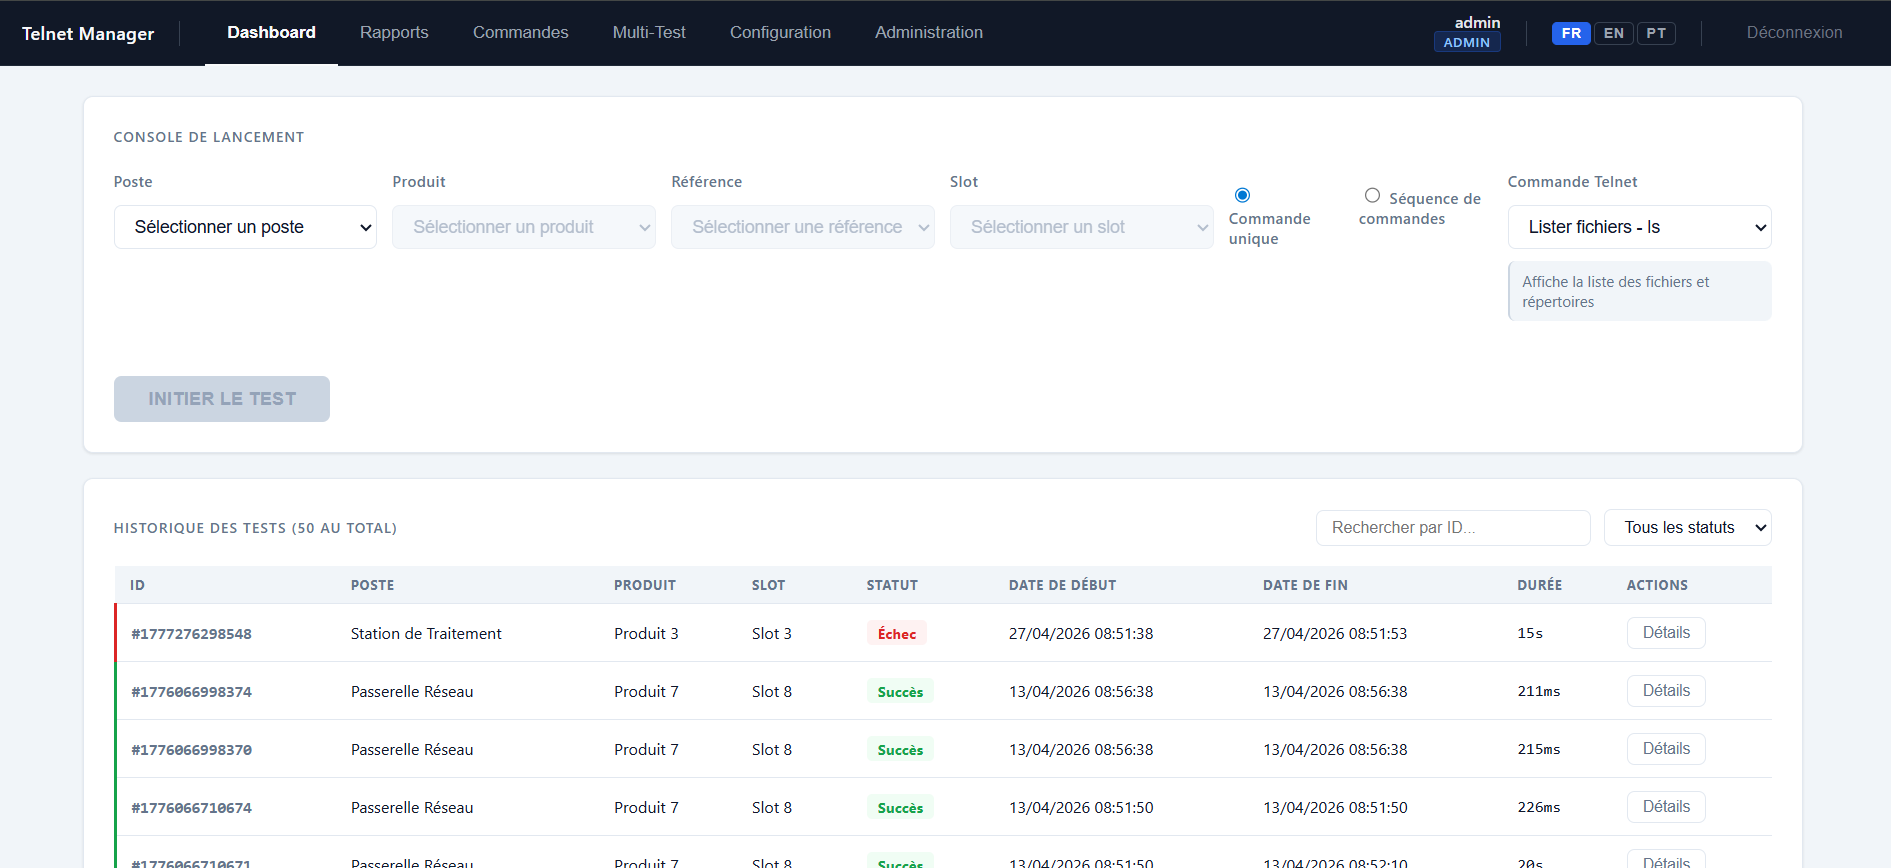
\includegraphics[width=\textwidth]{images/screen_dashboard}
  \caption{Capture d'écran~: Dashboard --- résultats en temps réel}
  \label{fig:screen_dashboard_live}
\end{figure}

\subsection{Gestion des équipements}

Le composant \texttt{Configuration.tsx} implémente la navigation
hiérarchique en onglets (Postes, Produits, Slots, Références). Chaque
onglet affiche un tableau paginé avec les opérations CRUD~:
\begin{itemize}
  \item \textbf{Ajouter}~: ouverture d'un formulaire modal avec
        validation côté client~;
  \item \textbf{Modifier}~: pré-remplissage du formulaire avec les
        données existantes~;
  \item \textbf{Supprimer}~: confirmation avant envoi de
        \texttt{DELETE /\{resource\}/:id}.
\end{itemize}

\begin{figure}[H]
  \centering
  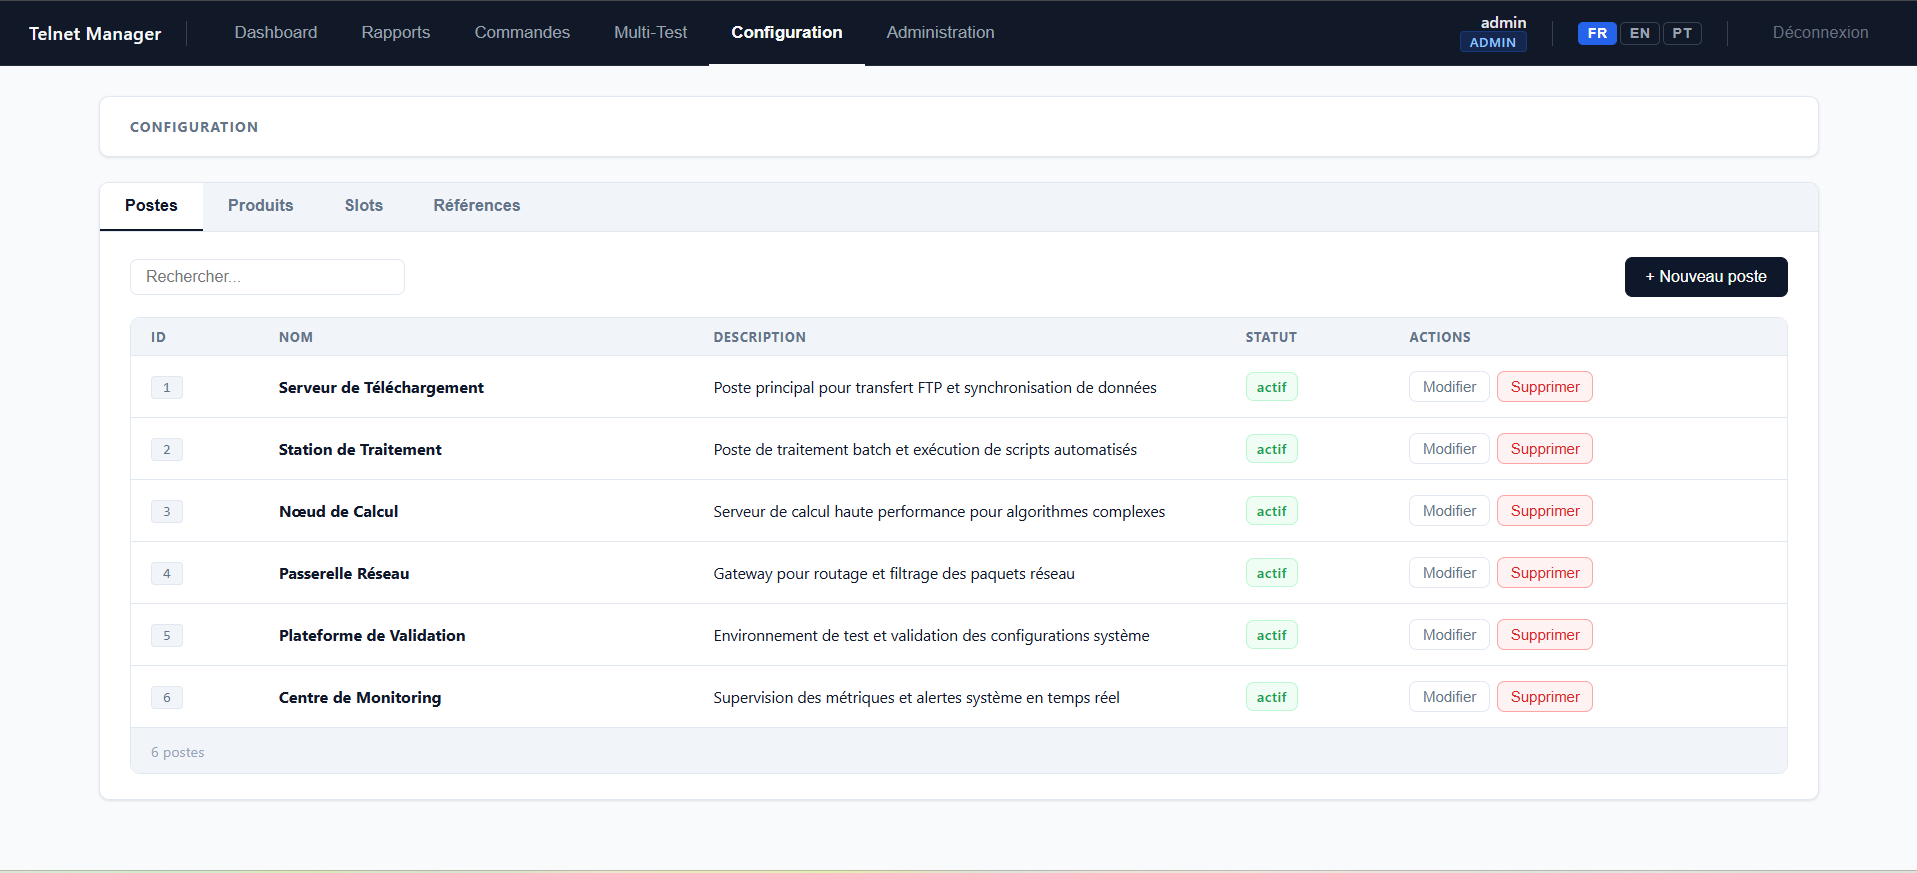
\includegraphics[width=\textwidth]{images/screen_config}
  \caption{Capture d'écran~: module de configuration --- gestion des slots}
  \label{fig:screen_config_slots}
\end{figure}

\subsection{Monitoring temps réel}

Le composant \texttt{MultiTest.tsx} permet de sélectionner plusieurs
slots et de lancer des tests Telnet en parallèle. Chaque slot a son
propre terminal de résultats, mis à jour indépendamment via les
messages WebSocket.

\begin{figure}[H]
  \centering
  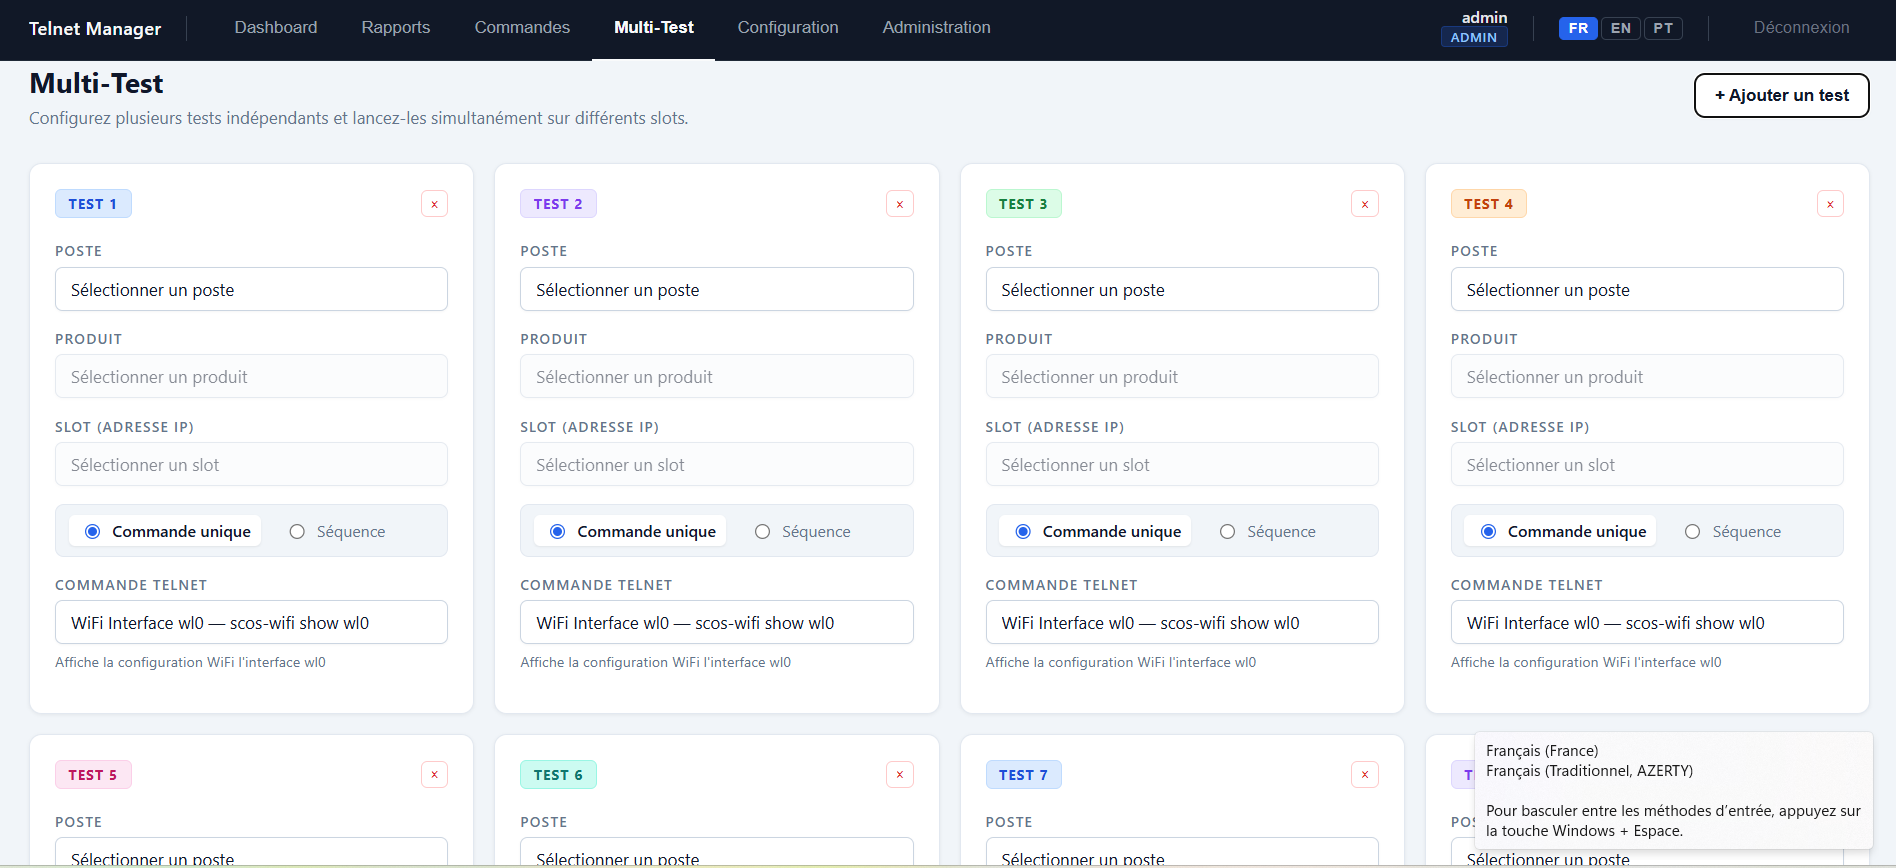
\includegraphics[width=\textwidth]{images/screen_multitest}
  \caption{Capture d'écran~: module MultiTest --- tests multi-slots en parallèle}
  \label{fig:screen_multitest_live}
\end{figure}

% -----------------------------------------------------------------
\section{Captures d'écran et démonstration}
% -----------------------------------------------------------------

\begin{figure}[H]
  \centering
  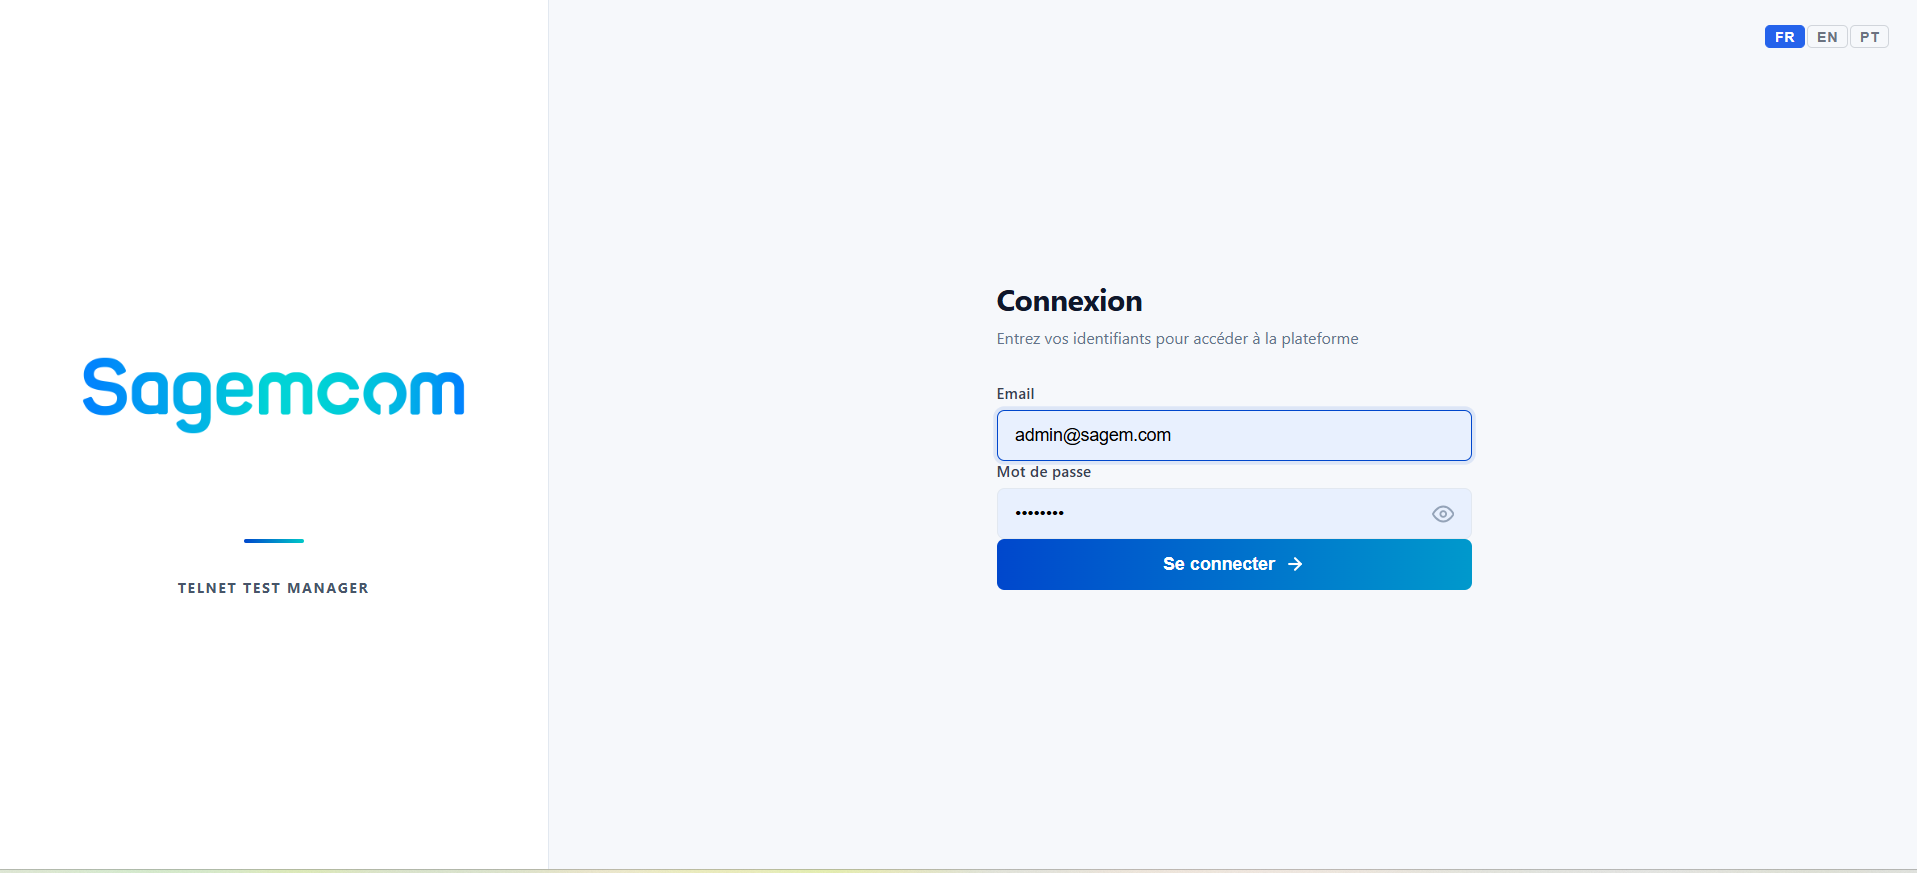
\includegraphics[width=0.75\textwidth]{images/screen_login}
  \caption{Capture d'écran~: interface d'authentification}
  \label{fig:screen_login}
\end{figure}

\begin{figure}[H]
  \centering
  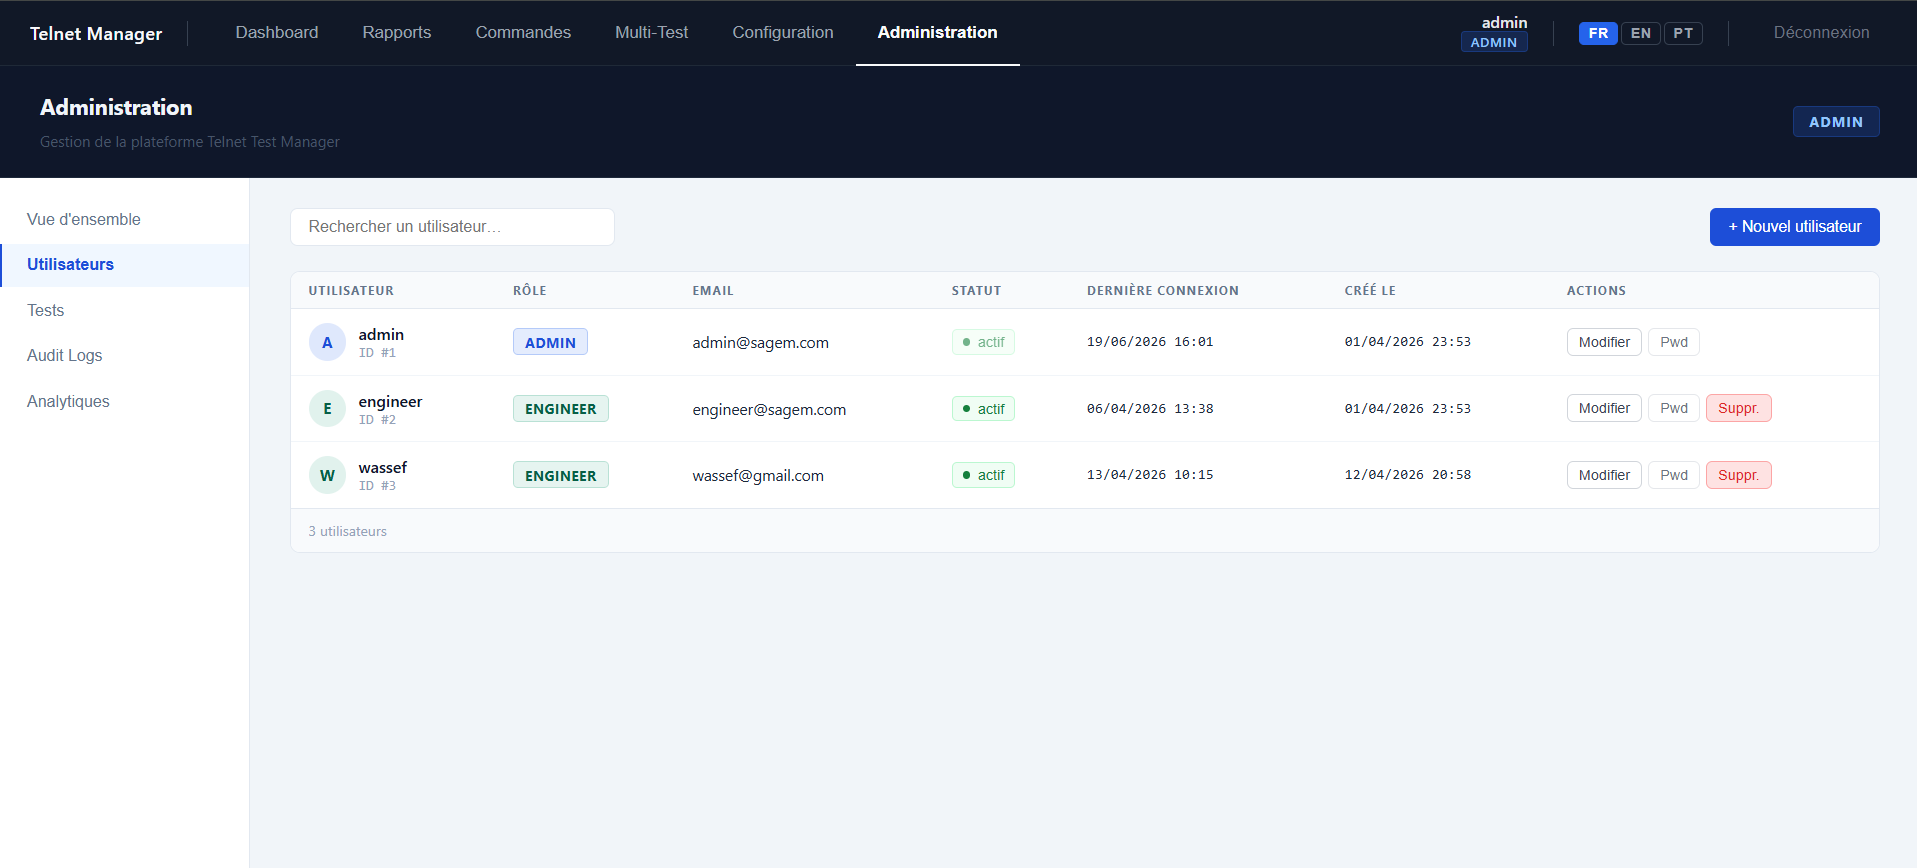
\includegraphics[width=\textwidth]{images/screen_admin}
  \caption{Capture d'écran~: panneau d'administration --- gestion des utilisateurs}
  \label{fig:screen_admin}
\end{figure}

\begin{figure}[H]
  \centering
  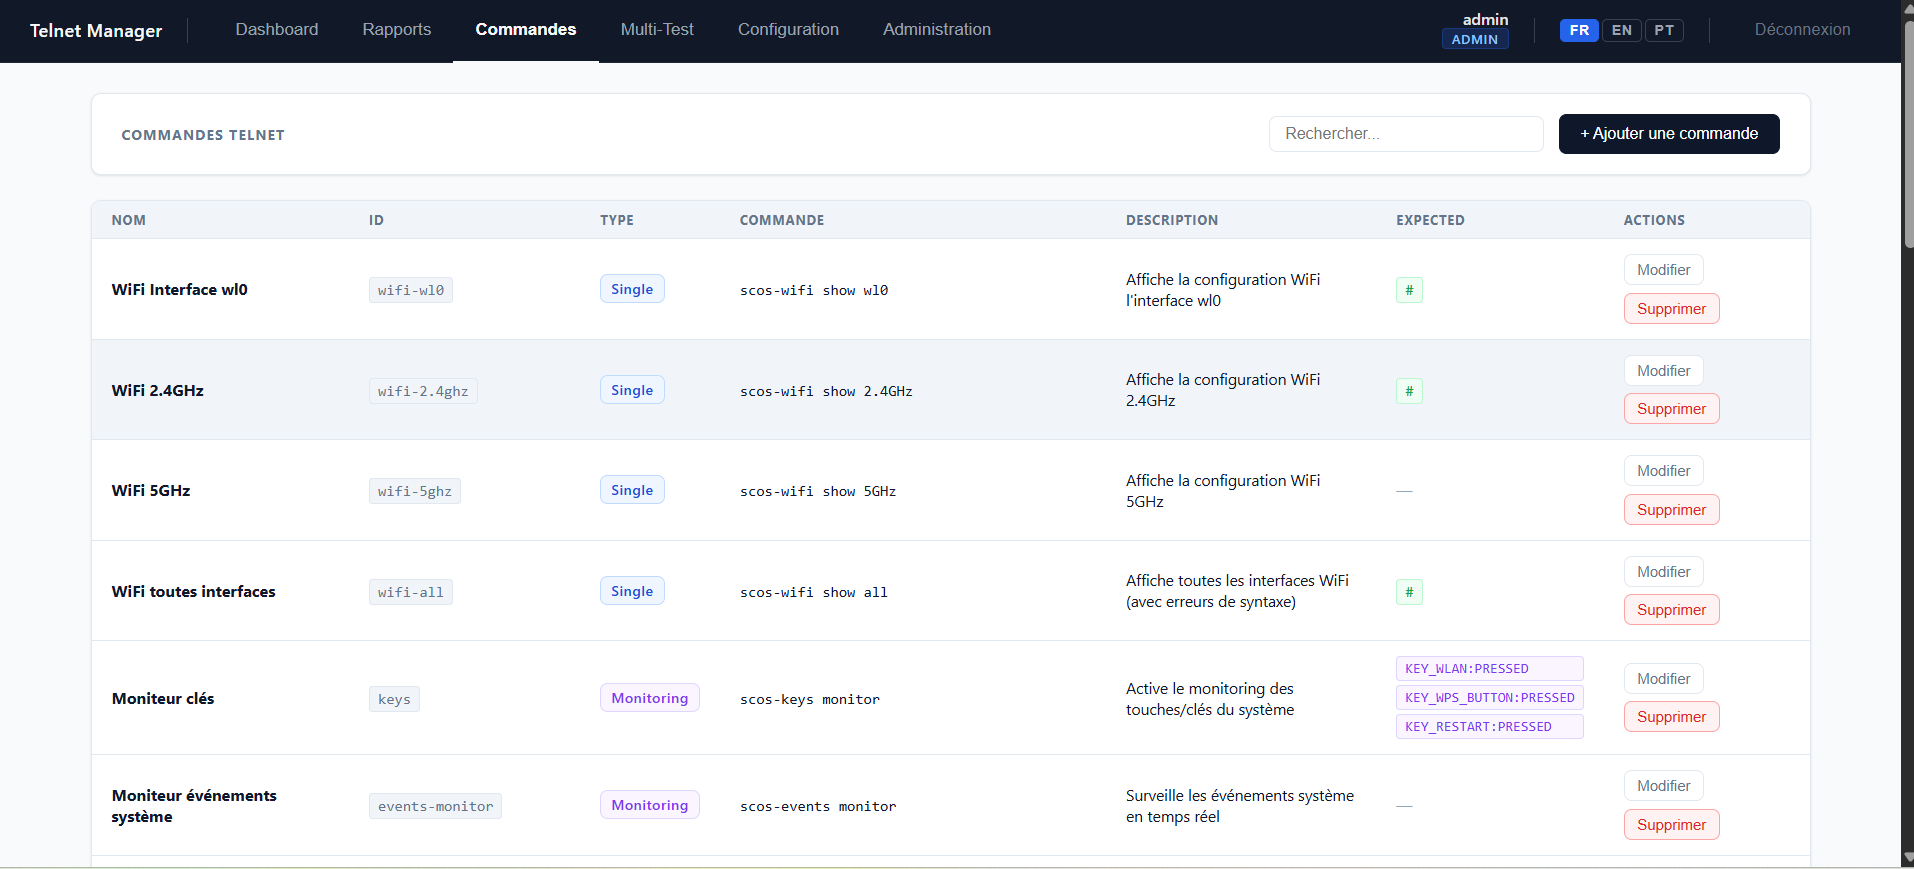
\includegraphics[width=\textwidth]{images/screen_commands}
  \caption{Capture d'écran~: bibliothèque de commandes Telnet}
  \label{fig:screen_commands}
\end{figure}

\begin{figure}[H]
  \centering
  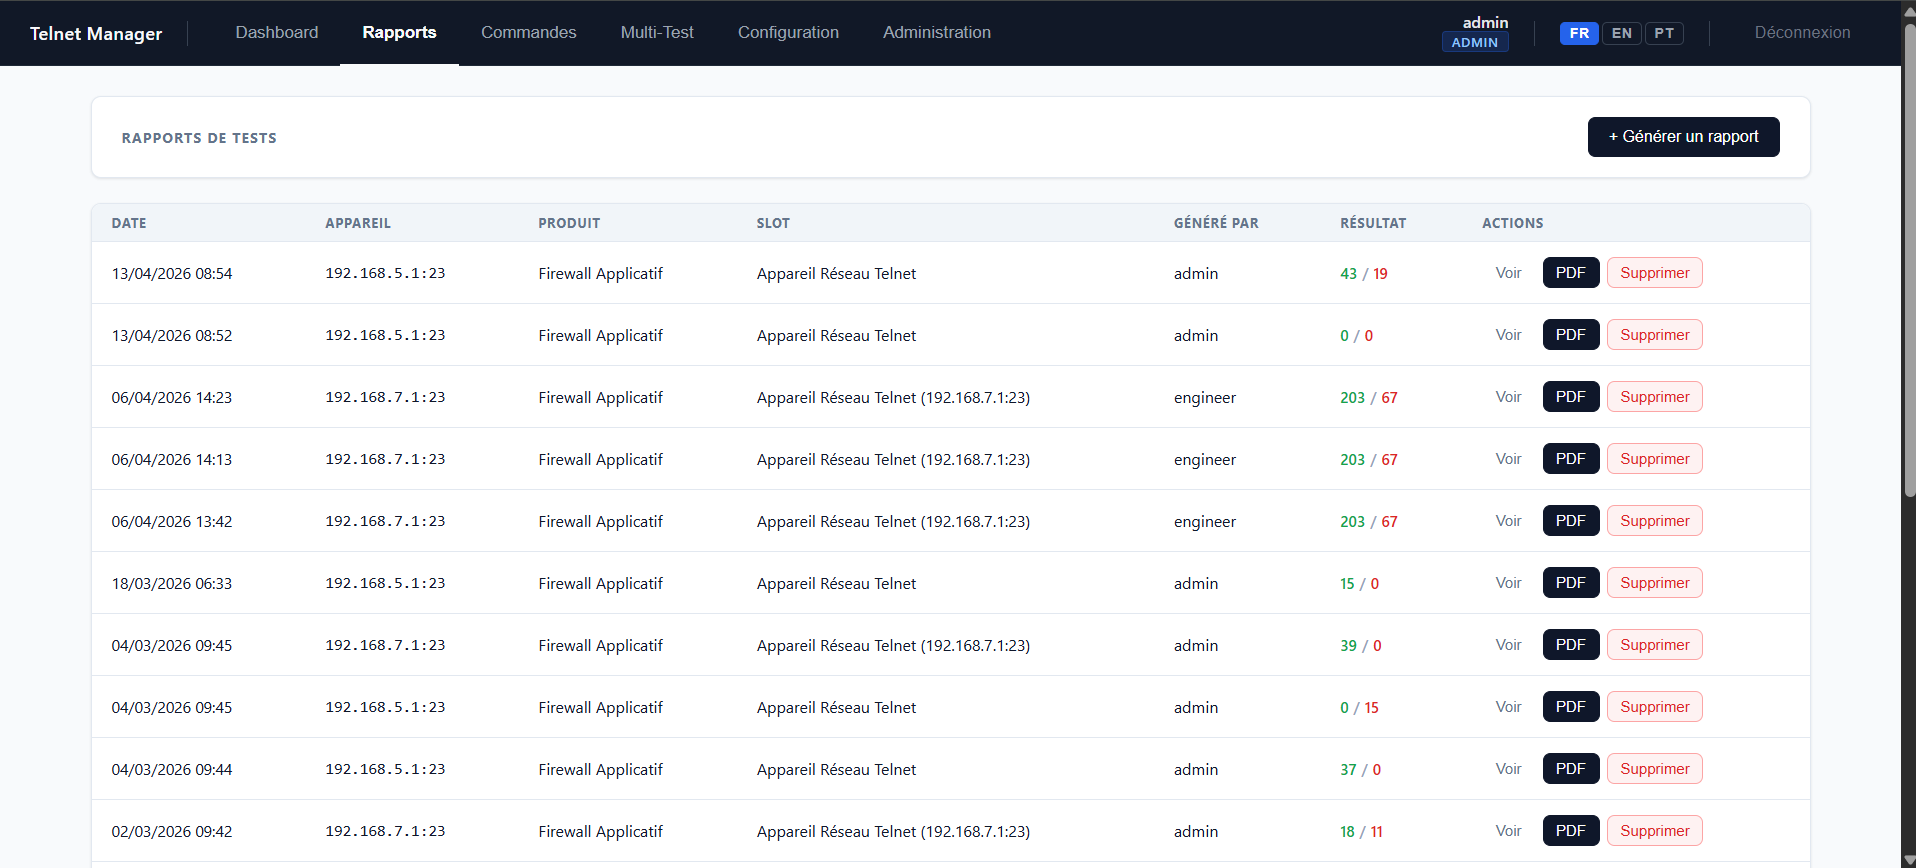
\includegraphics[width=\textwidth]{images/screen_reports}
  \caption{Capture d'écran~: module de génération de rapports}
  \label{fig:screen_reports}
\end{figure}

\begin{figure}[H]
  \centering
  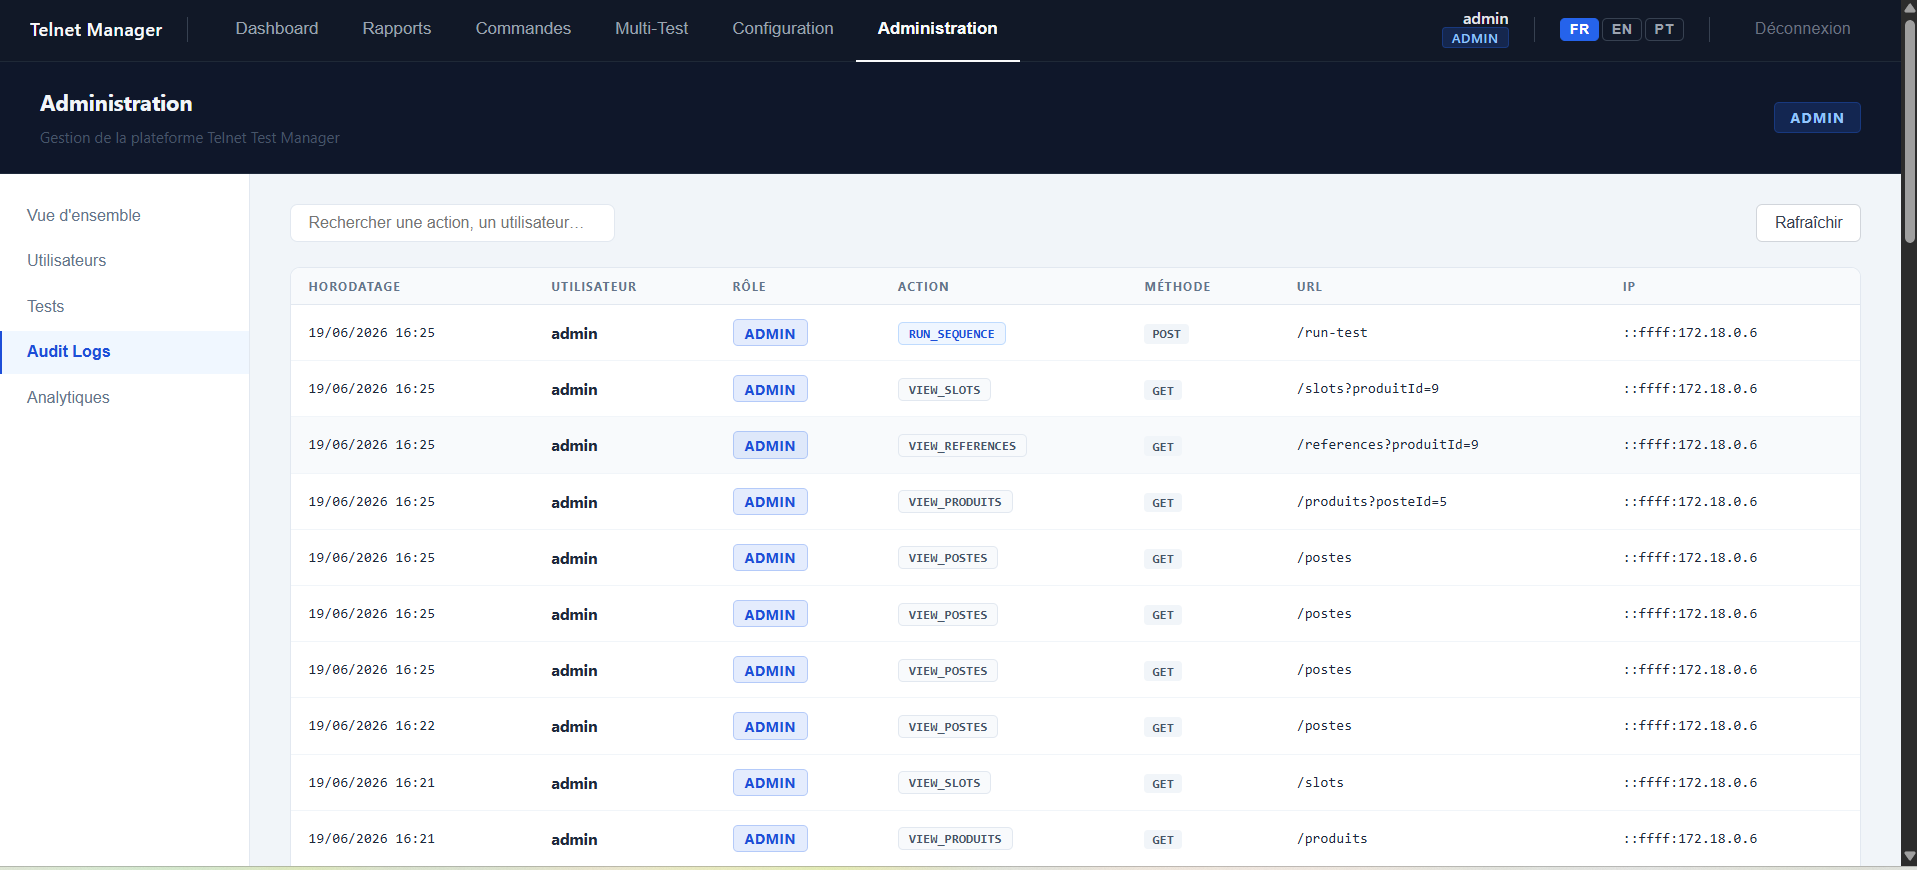
\includegraphics[width=\textwidth]{images/screen_auditlog}
  \caption{Capture d'écran~: journal d'audit --- traçabilité des actions utilisateurs}
  \label{fig:screen_auditlog}
\end{figure}

\section*{Conclusion}

Ce chapitre a couvert le développement des composants principaux de
Telnet Test Manager. Le moteur Telnet basé sur les Worker Threads assure
le non-blocage et le parallélisme. La Clean Architecture maintient une
séparation nette des responsabilités. Les 32 endpoints REST et la
connexion MongoDB forment la base de l'application. Le chapitre suivant
traite du déploiement et de l'infrastructure DevOps.
